% Este archivo es parte de la memoria del proyecto fin de carrera
% de Aarón Bueno Villares. Protegida bajo la licencia GFDL.
%
% Para más información, la licencia completa viene incluida en el
% fichero fdl-1.3.tex

% Copyright (C) 2010 Aarón Bueno Villares

\section{Principales problemas de implementación}
\label{sec:implementacion}

En este capítulo se abordarán algunas cuestiones de implementación
que, por su dificultad (e importancia asociada), merecen una atención
especial, o al menos, el deseo del autor de merecer una atención
especial.

Nos estamos refiriendo a problemas de implementación
funcional, es decir, de implementación a la hora de establecer un
cómputo que calcule a una función que resuelva un problema, y no a problemas de implementación
estructural, es decir, encargados de organizar los datos con los que
se trabajará y de asignar responsabilidades. Estos últimos ya han sido comentados en el capítulo de
análisis y diseño.

El asunto que forma base de \gom a nivel de reglas, es su
geometría. En \gom todo se reduce a figuras geométricas: las unidades
son rectángulos, al igual que el escenario; sus pivotajes y la visión se reducen a
problemas dentro y entre circunferencias, y, como veremos, los problemas mas importantes
del juego se reducen todos también a problemas geométricos.

Particularmente, estos problemas, como se ya se ha indicado, se resuelven
con la clase \emph{Gestor de escenario}, pues estos problemas
están ligados a la relación entre las distintas unidades presentes en
el escenario.

Tendremos una sección dedicada a los problemas que, para mí, han
resultado mas singulares sobre todo por su transfondo matemático en la
resolución. Existen otros
problemas que tampoco han sido fáciles de resolver a lo largo del
código. Por ejemplo, la
implementación de la clase \emph{Lista texto} o la resolución de los
combates en \emph{Gestor de combates}, debido a su ``\emph{desorden}''
conceptual (una amalgama de datos interrelacionados que hay que
manejar a la vez), son un ejemplo de aquellos problemas para nada
inmediatos a los que me he tenido que enfrentar. Pero la naturaleza de
estos problemas es fundamentalmente discreta, y encontrar su correcta
solución solo merece la observación atenta de sus partes sin la
necesidad de recurrir al ingenio ni a herramientas conceptules
externas.

En su lado extremo, tenemos los problemas como la caraterización de la
visión o el pivotaje máximo de una unidad, cuya resolución no es
\emph{a priori} intuitiva (ni \emph{a posteriori} tampoco).

\subsection{Pertenencia de un punto a una figura}
Para encontrar si el usuario ha hecho click en un icono, ha
seleccionado una unidad, si la esquina superior derecha de una unidad
está dentro del área de pivotaje de otra que desea moverse, o si la
intersección de dos rectas pertenece a un segmento, se hace necesario
disponer de dicha función para todas las estructuras geométricas a las
que sean aplicables (es decir, a todas).

Podemos encontrarnos con que necesitamos saber si un punto pertenece a una
recta, a una semicircunferencia o a un rectángulo con cualquier
orientación, por ejemplo. Para los casos en los que la figura
geométrica es descrita por una ecuación, su resolución es sencilla:
basta con ver si se verifica la ecuación de la figura sustituyendo en
ella la coordenada $x$ e $y$ del punto. Éste es el caso de la
pertenencia de un punto a una recta o a una circunferencia.

En el caso de la semicircunferencia, se traza una recta desde su
origen hasta el punto en cuestión, y si el ángulo de esta recta está
comprendida entre la de las dos rectas que definen a los extremos de
la semicircunferencia, y la longitud de dicha recta es menor a su
radio, el punto pertenece a la semicircunferencia, por lo tanto su
resolución también es bastante simple.

Pero para el caso de un rectángulo, que tampoco tiene ninguna ecuación
que lo defina, el problema se complica.

Podriamos pensar en trazar una recta desde cualquiera de sus vértices
hasta el punto en cuestión, he intentar ver si dicho segmento pertenece
al área del rectángulo, pero eso sencillamente es otra versión quizás mas
general del problema de la pertenencia de un punto a la
figura. También se podrían trazar cuatro segmentos, uno desde cada
vértice, y caracterizar los ángulos de cada pareja de segmentos. O la
suma de sus longitudes. Pero la solución que hemos adoptado es
computacionalmente mas sencilla, y esta basada en construir triángulos
alrededor de un punto.

\subsubsection{Orientación de un triángulo}
Imaginemos un triángulo $ABC$. Diremos que este triángulo tiene
orientación positiva si, al leer sus puntos en el plano en el orden
dado, se consigue una dirección horaria, y en caso contrario, su
orientación será negativa.

\begin{center}
\begin{tabular}{cc}
\begin{tikzpicture}[scale=2, decoration = {
    markings,
    mark=at position .10 with {\arrow[red, line width = 1.5pt]{>};} ,
    mark=at position .43 with {\arrow[red, line width = 1.5pt]{>}} ,
    mark=at position .76 with {\arrow[red, line width = 1.5pt]{>};} }
  ]
  \draw[gray,postaction={decorate}] (0,0) circle (1cm);
  \draw[thick,blue] (120:1cm) -- (240:1cm) -- (360:1cm) -- cycle;
  \filldraw[green] (120:1cm) circle(1pt);
  \filldraw[green] (240:1cm) circle(1pt);
  \filldraw[green] (360:1cm) circle(1pt);
  \draw (120:1.2cm) node[fill=white] {$A$};
  \draw (240:1.2cm) node[fill=white] {$B$};
  \draw (360:1.2cm) node[fill=white] {$C$};
\end{tikzpicture}
&
\begin{tikzpicture}[scale=2, decoration = {
    markings,
    mark=at position .10 with {\arrow[red, line width = 1.5pt]{<};} ,
    mark=at position .43 with {\arrow[red, line width = 1.5pt]{<}} ,
    mark=at position .76 with {\arrow[red, line width = 1.5pt]{<};} }
  ]
  \draw[gray,postaction={decorate}] (0,0) circle (1cm);
  \draw[thick, blue] (180:1cm) -- (300:1cm) -- (60:1cm) -- cycle;
  \filldraw[green] (180:1cm) circle(1pt);
  \filldraw[green] (300:1cm) circle(1pt);
  \filldraw[green] (60:1cm) circle(1pt);
  \draw (180:1.2cm) node[fill=white] {$A$};
  \draw (300:1.2cm) node[fill=white] {$C$};
  \draw (60:1.2cm) node[fill=white] {$B$};
\end{tikzpicture}
\end{tabular}
\end{center}

En este caso, vemos como la primera figura muestra una orientación
negativa (según nuestro convenio adoptado), por ir en sentido
antihorario, mientras que la segunda figura muestra una orientación
positiva al ir a favor de las agujas del reloj, según la lectura de
los vértices $A$, $B$ y $C$.

El motivo está muy relacionado con la regla que nos enseñaban en el
colegio de la mano derecha o del sacacorchos, aunque nosotros hemos
invertido su polaridad (por comodidades en la implementación). Si
giramos la mano en la
misma dirección que la que nos dicta el orden de lectura de los
vértices, si su sentido es anti-horario, será como sacar un
sacacorchos. Y lo opuesto si su sentido es horario.

Esta es consecuencia directa del producto vectorial de dos vectores en
un plano. Imaginemos que, en un espacio tridimensional, tenemos dos
vectores $\vec{u}$ y $\vec{v}$ en el plano $z=0$, es decir, que
$\vec{u} = ( u_x, u_y, 0)$ y $\vec{v} = (v_x, v_y, 0)$.

Si desarrollamos matemáticamente el producto vectorial en nuestras
condiciones, y tomando $\vec{u} = B - A$ y $\vec{v} = C - A$ para caracterizar al
triángulo $ABC$, tenemos:

\[ \vec{u} \times \vec{v} = 
  \begin{vmatrix}u_y & 0 \\v_y & 0 \\\end{vmatrix} \vec{i}
  - \begin{vmatrix}u_x & 0 \\v_x & 0 \\\end{vmatrix} \vec{j}
  + \begin{vmatrix}u_x & u_y \\v_x & v_y \\\end{vmatrix} \vec{k}
 = (u_xv_y - u_yv_x)\vec{k} = p\vec{k} \]

Como $\vec{k}$ es el vector de la base ortonormal correspondiente al
eje $z$, cuando $p>0$, significará que el producto vectorial crece por
el eje $z$, es decir, que la orientación del triángulo es antihoraria,
y bajo nuestro convenio, su orientación será negativa. En caso
contrario, será positiva.

Mas esquemáticamente:

\[orientacion(ABS) = \left\{
  \begin{array}{lc}
    positiva & |\vec{u}\times\vec{v}| \leq 0\\
    negativa & |\vec{u}\times\vec{v}| > 0\\
\end{array} \right. \]

Cuando el módulo del producto vectorial es 0, significa que los tres
puntos se encuentran en una misma linea recta. Consideraremos en este
caso que su orientación también es positiva dado que usaremos este resultado para
verificar que un punto pertenezca a la figura.

\subsubsection{Pertenencia de un punto a un rectángulo}
Ahora que sabemos caracterizar la orientación de un triángulo respecto
a sus vértices, veremos como podemos aplicar estos resultados al
problema de la pertenencia de un punto en un rectángulo (y en general,
en cualquier poliedro).

\begin{minipage}[h]{0.4\columnwidth}
\centering
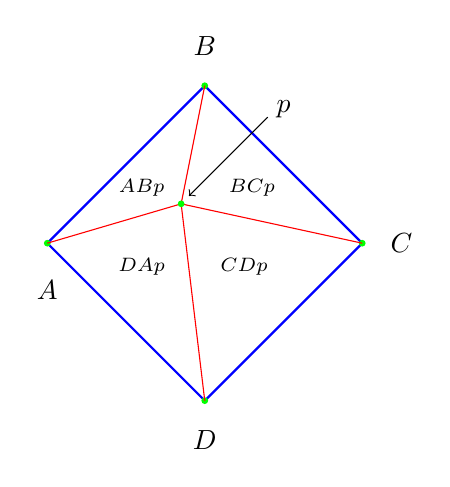
\begin{tikzpicture}
\draw[thick,blue] (0,0) -- (2,2) -- (4,0) -- (2,-2) -- cycle;

\filldraw[green] (0,0) circle(1pt);
\filldraw[green] (2,2) circle(1pt);
\filldraw[green] (4,0) circle(1pt);
\filldraw[green] (2,-2) circle(1pt);

\draw (0,-0.6) node {$A$};
\draw (2,2.5) node {$B$};
\draw (4.5,0) node {$C$};
\draw (2,-2.5) node {$D$};

\draw (3,1.7) node[fill=white] {$p$};
\draw[->] (2.8,1.6) -- (1.8,0.6);

\draw [red] (0,0) -- (1.7,0.5);
\draw [red] (2,2) -- (1.7,0.5);
\draw [red] (4,0) -- (1.7,0.5);
\draw [red] (2,-2) -- (1.7,0.5);

\filldraw[green] (1.7,0.5) circle(1pt);

\draw (1.2,0.7) node {$\scriptstyle ABp$};
\draw (2.6,0.7) node {$\scriptstyle BCp$};
\draw (2.5,-0.3) node {$\scriptstyle CDp$};
\draw (1.2,-0.3) node {$\scriptstyle DAp$};
\end{tikzpicture}
\end{minipage}
\begin{minipage}[h]{0.6\columnwidth}
La idea general es la siguiente: si un punto pertenece a una figura, y
construimos distintos triángulos con ese punto como uno de sus
vértices, la orientación de todos estos triángulos formados debe ser
la misma.

Por ejemplo en la figura de la izquierda, vemos como es importante el
orden en que se escogen los vértices de los triángulo. Deben escogerse
de modo que, si el punto efectivamente pertenece a la figura, todas
las orientaciones sean la misma, y en concreto, positiva. Para ello,
siempre hemos construido los triángulos en sentido horario y con el
punto $p$ como tercer vértice.
\end{minipage}

 Si por
ejemplo el segundo triángulo fuera $CBp$ en vez de $BCp$, el módulo de
su producto vectorial sería positivo, y por lo tanto su orientación
negativa, y nuestro método no funcionaría: el resto de triángulos
tendría una orientación positiva, sus orientaciones serían distintas,
y se nos indicaría que el punto no pertenece a la figura, lo cual es
falso.

Aquí se hace evidente por qué decidimos dar una orientación positiva
al caso $|\vec{u}\times\vec{v}| = 0$. En este caso, en nuestra
construcción de la figura, implicaría que el punto $p$ pertenece a una
arista (la correspondiente al triángulo construido actualmente) o
incluso a un vértice, y un punto que pertenece a una arista o un
vértice de la figura pertenece a la propia figura.

Es fácil ver como este método es aplicable directamente a cualquier
problema de pertenencia de un punto a un poliedro, su cálculo es muy
sencillo y computacionalmente es muy óptimo, pues su coste asintótico
es lineal respecto al número de vértices de la figura (dado que para
$n$ vértices, hay que construir $n$ triángulos y calcular el sentido
de cada uno de ellos).

Este problema me resulta importante por ser el primer problema
geométrico con el que me tuve que enfrentar en el juego, preparando
terreno para lo que vendría a continuación. Tras esto, se creó un
conjunto de estructuras y funciones que resolvían muchos otros
problemas geométricos necesarios, algunos sencillos de crear y otros
necesitando calma y tiempo para encontrar una solución correcta y
potente; cabe mencionar aquí el trato de rectas (caracterizadas como
hiperplanos) y el trato con circunferencias (sobre todo sobre la
intersección de circunferencias).

\subsection{Capacidades de movimiento actual}
El mundo de la intersección vino a tomar forma viva en este
problema. Tenemos tres casos del mismo: movimiento \emph{rect} máximo,
pivotaje derecho máximo, y pivotaje izquierdo máximo.

Tales problemas vienen delimitados por una máxima: no podrás acercarte
a menos de 10 unidades de terreno (véase reglamento) de otra unidad, sea amiga o
enemiga, y esto añade una dificultad interesante en el caso de los
pivotajes.

\subsubsection{Desplazamiento máximo}
En este problema se debe conseguir saber cual es la longitud máxima
que puede desplazarse una unidad en linea recta. Una unidad dispone de
un desplazamiento máximo de partida, y se ha de saber si existen
unidades en el camino que dificulten recorrer ese desplazamiento
máximo, teniendo en cuenta la distancia de respeto de 10 unidades de
terreno de juego entre unidades del mismo o distinto bando.

El problema se caracteriza de la siguiente forma: se construye un
rectángulo que tenga por ancho el frente de la unidad, y por alto, el
desplazamiento máximo de la unidad. Ahora se ha de ver qué unidades
enemigas tienen intersección con ese rectángulo (una unidad no es más
que otro rectángulo que caracteriza su ubicación), e ir calculando el
rectángulo libre de máxima altura a partir del rectángulo original.

Dos figuras pueden estar en posición una respecto a la otra de las
siguientes formas:
\begin{itemize}
\item Figuras disjuntas: cuando no tienen intersección.
\item Figuras contenidas: cuando su intersección es uno de los dos
  rectángulos.
\item Figuras cruzadas: cuando los vértices de su intersección no son
  vértices de ninguno de los dos rectángulos.
\item Figuras secantes: cuando su intersección contiene vértices
  de alguno de los dos rectángulos.
\end{itemize}

Esta taxonomía es importante por los siguientes motivos:
\begin{itemize}
\item Si buscamos vértices de otra figura, que pertenezcan a un
  dada, estoy encontrando figuras secantes y contenidas.
\item Si busco intersecciones de aristas, encuentro figuras secantes y cruzadas.
\item En caso contrario, las figuras son independientes.
\end{itemize}

Además, partimos del hecho de que la unidad de origen es una figura
\emph{bien colocada}. Con esto quiero decir que como partida la unidad
es disjunta a cualquier otra, y además, con 10 unidades de terreno de
separación, por lo tanto, el rectángulo de desplazamiento no estará
nunca contenida en ninguna otra figura, y nunca tendré que buscar que
sus vértices pertenezcan a las restantes.

\begin{minipage}[h]{0.4\columnwidth}
\centering
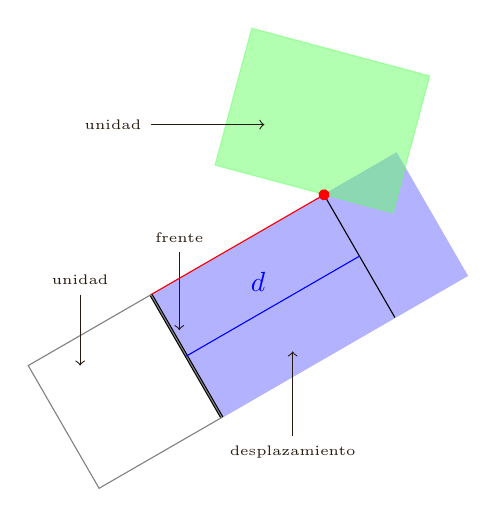
\begin{tikzpicture}[scale=1.8]
\filldraw[rotate=300,blue!30] (0,0) -- (1,0) -- (1,2) -- (0,2) --
cycle;
\filldraw[rotate=300,very thick] (0,0) -- (1,0);
\draw[brown!20!black,->] (.2,.3) node[above] {\tiny{frente}} -- (0.2,-.25);
\filldraw[rotate=345,opacity=.5, green!60] (0.2,1) -- (1.5,1) -- (1.5,2) -- (0.2,2) -- cycle;
\draw[rotate=300,gray,thin] (0,0) -- (1,0) -- (1,-1) -- (0,-1) --
cycle;
\draw[rotate=30,red] (0,0) -- (1.41,0);
\draw[rotate=30,black] (1.41,0)  -- (1.41,-1);
\draw[rotate=30,blue] (0,-0.5) -- (1.41,-0.5);
\draw[rotate=30,blue] (0.7,-0.3) node {$d$};
\filldraw[red,rotate=30] (1.41,0) circle(1pt);
\draw[brown!20!black,->] (-.5, 0) node[above] {\tiny{unidad}} -- (-.5, -.5);
\draw[brown!20!black,->] (1,-1) node[below] {\tiny{desplazamiento}}  --
(1,-.4);
\draw[brown!20!black,->] (0,1.2) node[left] {\tiny{unidad}} -- (.8,1.2);
\end{tikzpicture}
\end{minipage}
\begin{minipage}[h]{0.6\columnwidth}
Como podemos observar en la figura de la izquierda, para una unidad y
una arista concreta, hallamos la distancia de la
intersección entre la arista izquierda del área de desplazamiento y la
arista de la unidad \emph{enemiga}, hasta el frente de la unidad a
desplazar. Esa distancia será una cota máxima de desplazamiento
durante el resto del proceso de búsqueda.

Y este procedimiento se ejecuta para cada intersección entre cada
arista de cada unidad enemiga y las dos aristas verticales del área de
desplazamiento, y para cada vértice dentro del área de desplazamiento,
buscando el conflicto de menor distancia hasta el frente. También
ejecutamos estas operaciones con los bordes del escenario.
\end{minipage}

Hace falta advertir que al principio del proceso de búsqueda, se
ensancha virtualmente la unidad a desplazar un total de 10 unidades de
terreno, a lo ancho y a
lo alto, para respetar la distancia entre unidades de forma intrínseca
a la búsqueda.

\subsubsection{Pivotaje máximo}
De forma análoga al caso anterior, para calcular el pivotaje máximo
(por ejemplo, el pivotaje izquierdo -es decir, manteniendo como eje de
giro la esquina superior izquierda de la unidad-) ejecutamos de forma
similar al problema anterior, pero esta vez, en vez de trabajar con rectángulos, se trabaja
con una semicircunferencia que marca el pivotaje máximo inicial, y a
partir de ahí, reducimos el posible ángulo de giro a medida que se
encuentren intersecciones con otras unidades.

Pero como dijimos antes, aquí el hecho de engrosar a la unidad 10
unidades de terreno no nos da ninguna ventaja, y esta restricción hay
que cuidarla explícitamente en el proceso de búsqueda. El hecho de que
no nos de ninguna ventaja es debido a que, primeramente, el radio de
la semicircunferencia de partida no es el ancho de la unidad, sino su
diagonal.

Dado que al desplazar la unidad, hay que tener en cuenta el terreno
que este ocupa, también por ello hay que considerar la esquina opuesta al
eje de pivotaje, que siempre quedará fuera de dicha
semicircunferencia, como se aprecia en la figura inferior.

Por ello, como se ve en el gráfico, el área correcta de consideración es la
semicircunferencia de radio igual a la diagonal de la unidad. Y esta
diagonal no tiene ninguna relación ni proporción directa con las diez
unidades de terreno que se intentan respetar ensanchando a la unidad.

\begin{minipage}[h]{.5\columnwidth}
Por otro lado, ahora estamos calculando ángulos, no distancias. Un
incremento de 10 unidades de terreno en altura, son las 10 unidades de
terreno que hay que respetar si el movimiento es recto. Pero como
ahora tratamos con giros, un incremento de 10 unidades de terreno no
implican una distancia de 10 unidades de terreno con el punto de
intersección de dicha semicircunferencia con otra unidad. Así que,
ahora debemos de recurrir a otra solución para conseguir ese
\emph{respeto}.
\end{minipage}
\begin{minipage}[h]{.5\columnwidth}
\centering
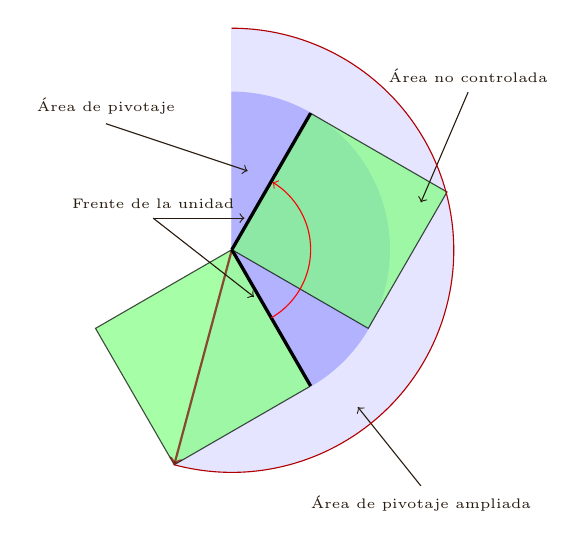
\begin{tikzpicture}[scale=2]
\filldraw[blue!10,rotate=300] (0,0) -- (1,-1) arc (-45:150:1.41cm) --
cycle;
\filldraw[opacity=.7,rotate=300,green!50,draw=black] (0,0) -- (1,0) --
(1,-1) -- (0,-1) -- cycle;
\draw[opacity=.7,red!50!black,rotate=300,thick,->] (0,0) -- (1,-1);
\filldraw[blue!30,rotate=300] (1,0) arc (0:150:1cm) -- (0,0) -- cycle;
\filldraw[very thick,rotate=300] (0,0) -- (1,0);

\filldraw[opacity=.7,rotate=60,green!50,draw=black] (0,0) -- (1,0) -- (1,-1) -- (0,-1) --
cycle;
\draw[red,->,rotate=300] (.5,0) arc (0:119:.5cm);
\filldraw[very thick, rotate=60] (0,0) -- (1,0);
\draw[brown!20!black,->] (-.8,.8) node[above] {\tiny{Área de pivotaje}}
-- (.1,.5);
\draw[brown!20!black,->] (1.2,-1.5) node[below] {\tiny{Área de pivotaje ampliada}}
-- (.8,-1);
\draw[brown!20!black,->] (1.5,1) node[above] {\tiny{Área no controlada}}
  -- (1.2,.3);
\draw[red!70!black,rotate=300] (1,-1) arc (-45:150:1.41cm);
\draw[brown!20!black,->] (-.5,.2) node[above] {\tiny{Frente de la unidad}}
  -- (.08,.2);
\draw[brown!20!black,->] (-.5,.2) -- (.14,-.3);
\end{tikzpicture}
\end{minipage}

\begin{minipage}[h]{0.5\columnwidth}
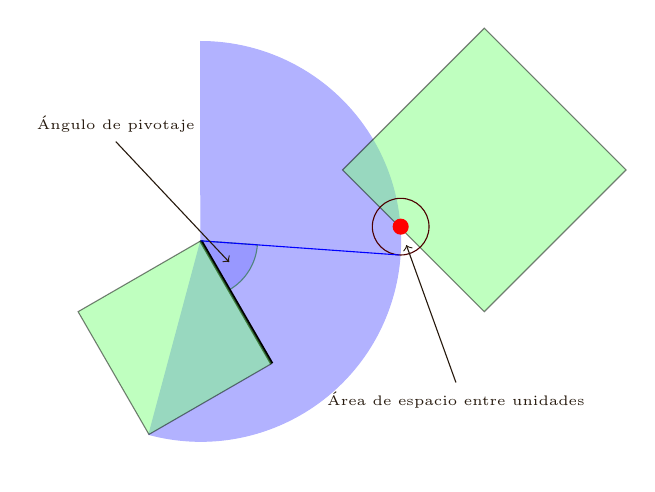
\begin{tikzpicture}[scale=1.8]
\filldraw[blue!30,rotate=300] (0,0) -- (1,-1) arc (-45:150:1.41cm) --
cycle;
\filldraw[opacity=.5,blue!50, draw=green!40!black,rotate=300] (.4,0) arc(0:56:.4cm) -- (0,0) -- cycle;
\draw[very thick, rotate=300] (0,0) -- (1,0);
\filldraw[opacity=.5,rotate=300,green!50,draw=black] (0,0) -- (1,0) --
(1,-1) -- (0,-1) -- cycle;
\filldraw[opacity=.5,green!50,draw=black] (1,.5) -- (2,1.5) --
(3,0.5) -- (2,-.5) -- cycle;
\filldraw[red] (1.41,.1) circle(1.5pt);
\draw[red!30!black] (1.41,.1) circle(.2cm);
\draw[blue] (0,0) -- (1.4,-.1);

\draw[brown!20!black,->] (1.8,-1) node[below] {\tiny{Área de espacio
    entre unidades}}-- (1.45,-.03);
\draw[brown!20!black,->] (-.6,.7) node[above] {\tiny{Ángulo de pivotaje}}-- (.2,-.15);
\end{tikzpicture}
\end{minipage}
\begin{minipage}[h]{0.5\columnwidth}
La solución adoptada es la siguiente: al igual que en el caso
anterior, para cada unidad, encontramos la intersección entre sus
aristas y la semicircunferencia de referencia de pivotaje, y también
los puntos que estén dentro de la figura. Y ahora, para cada punto,
trazamos una circunferencia de un radio de 10 unidades de
terreno. Luego tomamos los dos puntos de intersección entre dicha
circunferencia y la semicircunferencia de pivotaje: si se traza una
recta desde el origen de la semicircunferencia a dichos puntos, éstos
serán tangentes a la circunferencia \emph{de precaución}, y son éstos
puntos precisamente los que nos interesan.
\end{minipage}

De esta forma, buscamos el punto que nos de un ángulo de pivotaje
mínimo, y ese será el ángulo disponible de pivotaje actualmente.

Hay que advertir que, aunque nunca nos puede dar un ángulo
menor que 45º (puesto que la semicircunferencia de pivotaje tiene esta
cota mínima), si el valor está comprendido entre 0 y -45 (aunque
estrictamente hablando, esto no es un ángulo de pivotaje), significará
que la unidad no puede moverse porque si pivotara, entraría en
contacto con una unidad que está a su lado, pero no delante.

\subsection{Visión de una unidad}
Caracterizar la visión de una unidad, es decir, determinar qué unidad
ve a quién, es igual que caracterizar la
visión de una persona. Una persona ve un objeto cuando el espacio que
hay entre los dos está completamente libre. Si está parcialmente
ocupado también puede observarse dicho objeto, aunque la calidad de la
información que se recibe de dicho objeto es bastante menor. Si la parcialidad
de la obstaculización es muy alta, llegando a ocultar casi la
totalidad del objeto, se observará una figura de la que no
se reconocerá su forma, es decir, no se sabrá que objeto es.

Al principio, el problema de la caracterización de una unidad ignoraba
este último detalle tan importante y la vez tan simplificador. Se
intentó programar un algoritmo que admitiera una visualización directa
con tal de que el espacio no estuviera \emph{completamente}
ocupado. Es decir, que una sola recta infinitesimal de visión era
suficiente. La única forma de determinar tal tipo de visualización era
modificando el área de visión de partida.

Es decir, si partíamos de una semicircunferencia con centro en la
unidad y una amplitud de 120º de visión (siempre respecto al frente de
la unidad, porque es el frente el \emph{que ve}). Esta figura debe
entonces poderse modificar en otra figura de la complejidad que sea,
incluso dividirse en varias figuras disjuntas. Por ejemplo, un objeto
frente a la unidad de origen parte el área de visión en dos: la visión
correspondiente a los efectivos situados mas a la izquierda de la
unidad, y la visión correspondiente a los efectivos situados mas a la
derecha. Por tanto, determinar si la unidad objetivo es vista es
dividida en la determinación de la \emph{supervivencia} de dos
áreas. Si imaginamos todas las posibles situaciones nos damos cuenta
de que nos podemos encontrar ante cualquier tipo de partición y de
figura geométrica imaginable.

\begin{minipage}[h]{0.5\columnwidth}
Cuando se tuvo en cuenta el hecho de que, para observar un objeto, al
menos debe haber una franja continua de visionado, el problema se
simplificó de la siguiente forma: en vez de tener el problema de un
área modificable, y pretender que ese área nunca se haga nula (lo que
implicaría que no existe visibilidad), ahora lo resolvemos con un
descarte de áreas.

Cada área será lo que en la figura de nuestra derecha hemos llamado
\emph{haz de visión}. Un haz de visión es un rectángulo que comienza
en el frente de la unidad origen, y finaliza en una arista de la unidad de destino.
\end{minipage}
\begin{minipage}[h]{0.5\columnwidth}
\centering
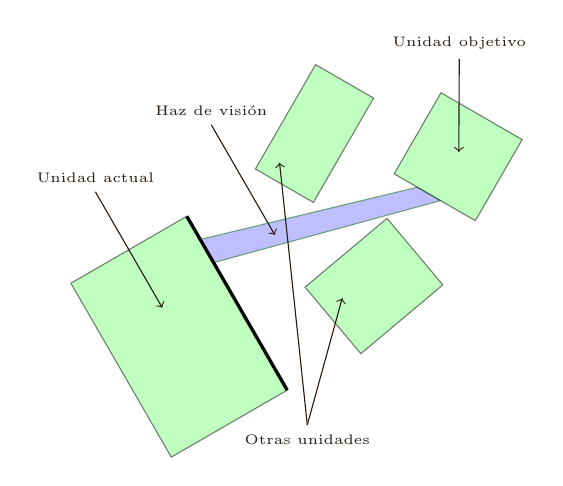
\begin{tikzpicture}[
  scale=1.7,
  rotate=300,
  unidad/.style={opacity=.5,green!50,draw=black},
  area/.style={opacity=.5,blue!50, draw=green!40!black},
  descripcion/.style={brown!20!black,->},
  ]
\coordinate (A) at (0,1);
\coordinate (B) at (1.5,1);
\coordinate (C) at (1.5,0);
\coordinate (D) at (0,0);

\coordinate (a) at (.5,2.5);
\coordinate (b) at (1.2,2.5);
\coordinate (c) at (1.2,3.2);
\coordinate (d) at (.5,3.2);

\coordinate (REF) at (a);
\coordinate (CENTRO) at (.75,1);

\filldraw[area] (0.4,1) -- (0.2,1) -- ({.5 + .2*cos(30)}, {2.5 + .2*sin(30)})--
+({.2*cos(30)}, {.2*sin(30)}) -- cycle;

\filldraw[unidad] (A) rectangle (C);

%No se por que no funciona girar coordenadas (c).
\filldraw[unidad,rotate around={30:(REF)}] (a) rectangle (1.2,3.2);

\coordinate (alfa) at (.9,1.5);
\coordinate (beta) at (1.4,2.4);

\filldraw[unidad,rotate around={10:(alfa)}] (alfa) rectangle (beta);

\filldraw[unidad,rotate around={30:(-.5,2.4)}] (0,1.5) rectangle
(-.5,2.4);

\draw[descripcion] (-.5,.5) node[above]{\tiny{Unidad actual}} --
(.5,.5);
\draw[descripcion] (-.5,1.5) node[above]{\tiny{Haz de visión}} --
(.45,1.5);

\coordinate (refunidades) at (1.8,1);

\draw[descripcion] (refunidades) node[below]{\tiny{Otras unidades}} --
(1.11,1.7);

\draw[descripcion] (refunidades) -- (0,1.8);

\draw[very thick] (A) -- (B);

\coordinate (refunidadobjetivo) at (0,3.35);

\draw[descripcion] (refunidadobjetivo) node[above]{\tiny{Unidad
    objetivo}} -- (.6,3);
\end{tikzpicture}
\end{minipage}

Tanto la base, en la unidad de origen, como su arista opuesta en la
unidad de destino, tienen un tamaño de 5 unidades de terreno, pues
esta ha sido la cota elegida para caracterizar la visión de una
unidad.

Lo que hacemos, en general, es crear todos los
posibles haces de visión entre la unidad origen y la unidad
objetivo. Esto entraña un problema. Por ejemplo, si nos fijamos en la
figura de referencia, la unidad de origen podrá ver, como mucho, dos
aristas de la unidad de destino. El nuevo problema que surge con este
planteamiento es el de caracterizar la arista o aristas
características de visión. Este problema se resuelve tal y como
muestra la siguiente figura.

\begin{minipage}[h]{0.4\columnwidth}
\centering
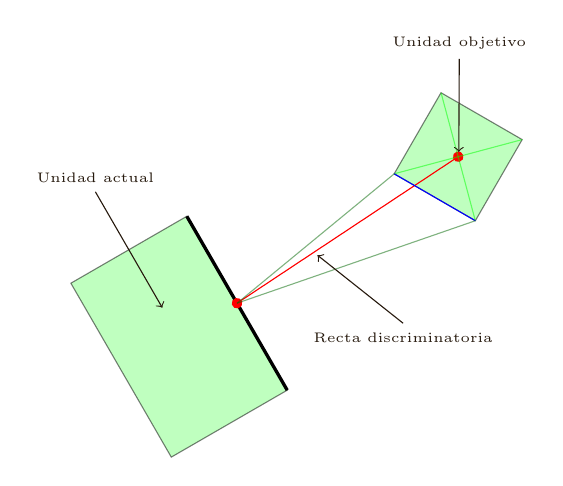
\begin{tikzpicture}[
  scale=1.7,
  rotate=300,
  unidad/.style={opacity=.5,green!50,draw=black},
  area/.style={opacity=.5,blue!50, draw=green!40!black},
  descripcion/.style={brown!20!black,->}
  ]
\coordinate (A) at (0,1);
\coordinate (B) at (1.5,1);
\coordinate (C) at (1.5,0);
\coordinate (D) at (0,0);

\coordinate (a) at (.5,2.5);
\coordinate (b) at (1.2,2.5);
\coordinate (c) at (1.2,3.2);
\coordinate (d) at (.5,3.2);

\coordinate (REF) at (a);
\coordinate (CENTRO) at (.75,1);

\filldraw[unidad] (A) rectangle (C);

%No se por que no funcioan girar coordenadas (c) no funciona.
\filldraw[unidad,rotate around={30:(REF)}] (a) rectangle (1.2,3.2);
\draw[very thick] (A)--(B);

\filldraw[red,rotate around={30:(REF)}] (CENTRO) circle(1pt) -- (intersection of a--1.2,3.2
and 1.2,2.5--.5,3.2) circle(1pt);
\draw[opacity=.5,green, rotate around={30:(REF)}] (a)--(1.2,3.2);
\draw[opacity=.5,green, rotate around={30:(REF)}] (1.2,2.5)--(.5,3.2);

\draw[blue, rotate around={30:(REF)}] (a)--(1.2,2.5);
\draw[area] (CENTRO)--(a);
\draw[area, rotate around={30:(REF)}] (CENTRO) -- (1.2,2.5);

\draw[descripcion] (-.5,.5) node[above]{\tiny{Unidad actual}} --
(.5,.5);

\coordinate (refunidadobjetivo) at (0,3.35);

\draw[descripcion] (refunidadobjetivo) node[above]{\tiny{Unidad
    objetivo}} -- (.6,3);

\draw[descripcion] (1.5,2) node[below]{\tiny{Recta discriminatoria}}
-- (.74, 1.7);
\end{tikzpicture}

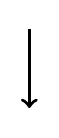
\begin{tikzpicture}
\draw[very thick, black, ->] (5,1) -- (5,0);
\end{tikzpicture}

\begin{tikzpicture}[
  scale=1.7,
  rotate=300,
  unidad/.style={opacity=.5,green!50,draw=black},
  area/.style={opacity=.5,blue!50, draw=green!40!black},
  descripcion/.style={brown!20!black,->},
  decoration = {
    markings,
    mark=at position .50 with {\arrow[red, line width = 1.5pt]{>};} }
  ]
\coordinate (A) at (0,1);
\coordinate (B) at (1.5,1);
\coordinate (C) at (1.5,0);
\coordinate (D) at (0,0);

\coordinate (a) at (.5,2.5);
\coordinate (b) at (1.2,2.5);
\coordinate (c) at (1.2,3.2);
\coordinate (d) at (.5,3.2);

\coordinate (REF) at (a);
\coordinate (CENTRO) at (.75,1);

\filldraw[area,opacity=.3,rotate around={30:(REF)}] (CENTRO) -- (.5,3.2) --
(1.2,2.5) -- cycle;
\filldraw[area,black!80,rotate around={30:(REF)}] (.5,3.2) --
(1.2,2.5) -- (1.2,3.2) -- cycle;

\filldraw[unidad] (A) rectangle (C);

%No se por que no funcioan girar coordenadas (c) no funciona.
\filldraw[unidad,rotate around={30:(REF)}] (a) rectangle (1.2,3.2);
\draw[very thick] (A)--(B);

\draw[red, rotate around={30:(REF)}] (1.2,2.5)--(.5,3.2);

\draw[blue, rotate around={30:(REF)}] (a)--(1.2,2.5);
\draw[blue, rotate around={30:(REF)}] (a)--(.5,3.2);
\draw[red, rotate around={30:(REF)},postaction={decorate}] (CENTRO) --
(1.2,2.5);

\draw[descripcion] (1.5,2) node[below]{\tiny{Área de referencia}}
-- (.74, 2);
\draw[descripcion] (0,3.5) node[above]{\tiny{Área oculta}} --
(.6,3.15);
\draw[descripcion] (-.27,1.4) node[above]{\tiny{Diagonal
    discriminatoria}} -- (.63,2.96);
\end{tikzpicture}
\end{minipage}
\begin{minipage}[h]{0.6\columnwidth}
Proyectamos, desde el centro del frente de la unidad de origen, un
segmento que acabe en el centro del rectángulo de la unidad de
destino. A esa recta la llamaremos recta discriminatoria. Esa recta
deberá intersecar con alguna arista de la unidad de
destino. A esa arista la llamaremos arista discriminatoria.

Luego, desde el centro del frente, proyectamos dos nuevos segmentos,
que acaben respectivamente en los extremos de la arista
discriminatoria. Nos quedamos, en este caso, con el segmento de mayor
longitud, situación que nos lleva a la segunda figura.

Una vez determinado el segmento mayor, elegimos la diagonal de la
unidad enemiga que coincida con su extremo con dicho segmento. A esta
diagonal la llamaremos, finalmente, diagonal discriminatoria.

Esta diagonal es importante porque divide a la unidad objetivo en dos
mitades, una que está frente a la unidad origen, y otra que
está \emph{oculta}. Las aristas que estén delante de la diagonal
discriminatoria serán las que queden descubiertas a la unidad
origen. Se puede observar como estas aristas están dentro del
\emph{área de referencia} que hemos construido proyectando el centro
del frente ha la diagonal discriminatoria.
\end{minipage}

Y ahora hacemos la última observación importante. Si intentamos
construir todos los haces de visión posibles con respecto a las
aristas descubiertas, y también, y ésta es la novedad, con respecto a la diagonal de
referencia, nos damos cuenta de que, con solo hacer que la unidad vea
a la diagonal de referencia, nos basta para admitir que ve a la unidad
original.

El método, pues, será explorar una a una todas las unidades de la
partida (de media, unas 10 o 15 unidades)
para cada rectángulo de referencia (que de media, serán entorno a unas
60), buscando intersecciones que descarten a dichos rectángulos, y, en
cuanto encontremos un haz de visión libre, abortamos la búsqueda y
admitimos que la unidad de origen vé a la unidad de destino.

\subsection{Movimiento de carga}
El movimiento de carga se resuelve de forma muy parecida al problema
de la visión, al menos en su planteamiento inicial. Evidentemente,
para cargar, la unidad tiene que ver a su objetivo. Y además, solo
podrá cargar a uno de los flancos que estén dentro de su 
visión. Y en este sentido, es donde se reenlaza este problema con el
anterior:

\begin{itemize}
\item Se obtienen las aristas \emph{descubiertas} vistas en la sección
  anterior.
\item Se buscan todas las posibles posiciones de carga en dichas
  aristas.
\item Se asegura que una posición sea accesible mediante una carga.
\item Se sigue buscando hasta encontrar una posición que también sea
  accesible, y que sea mejor, usando los criterios impuestos por el
  reglamento de \gom sobre los movimientos de carga.
\item Se desplaza la unidad a dicha posición.
\end{itemize}

Las distintas posiciones en las que es posible efectuar una carga
también es similar al caso anterior. En cada arista descubierta, voy
\emph{deslizando} un segmento del mismo tamaño que el frente de la
unidad, a intervalos de 5 en 5 unidades de terreno. Cada posición,
representa una posible posición de carga. Además, como los rangos de
ocupacion de las unidades son siempre múltiplos de 5, de esta forma se
exploran todas las posibles situaciones útiles.

Para calcular si el espacio de carga está disponible, sencillamente,
formamos un rectángulo como resultado de unir los extremos de ambos
segmentos: el frente de la unidad, y el nuevo frente virtual de la
nueva y posible posición de carga. Si dicho rectángulo está libre y si
además, la posición final también lo está, diremos que la carga es
posible. Luego tendremos que vigilar si existen mas posiciones de
carga que permitan enfrentar un número mayor de efectivos, o que se
recorra una distancia menor.

Si bien es cierto que el movimiento de carga real de la unidad no tiene
por qué coincidir con el área marcada por el rectángulo que formamos para su
representación, no nos hace falta tener en cuenta la posible área de
la unidad que pueda salirse de dicho rectángulo, por las siguientes razones:

\begin{itemize}
\item Los movimientos de carga son movimientos en partes libres y
  caóticos, y no se puede caracterizar en qué posición exacta estaría
  cada unidad en cada paso de la carga.
\item Las unidades, en la antigüedad, podían reorganizarse y
  pivotar suavemente al inicio de la carga, se podia perder levemente
  la rigidez de la formación 
  formación para hacer mas flexible su recorrido, etc. Con esto, la
  unidad tiene cierta flexibilidad a la hora de desplazar su carga,
  siendo dicho \emph{área de carga} rectángulas la mejor aproximación
  a su recorrido.
\item Y la última razón, y a su vez la mas importante, ninguna
  posición intermedia en este \emph{área de carga} será
  una posición final de la unidad, salvo la última, y la última sí que
  se comprueba.
\end{itemize}

\subsection{Movimiento de huida}
El movimiento de huida se puede ver como una variante del problema del
desplazamiento con la diferencia o particularidad de que el
desplazamiento, en vez de tener una cota máxima de movimiento, su cota
es mínima.

Es decir, en el caso del desplazamiento, se debía calcular cual era el
desplazamiento máximo que se podía realizar sin entrar en contacto con
ninguna otra unidad. En el caso del movimiento de la huida, el valor
de partida es el valor mínimo que hay que realizar, y si no hay
espacio, este valor se supera en busca de la primera posición de la
unidad que tenga el suficiente espacio libre como para que la unidad
que huye pueda \emph{estacionar}.

En general, el verdadero problema es caracterizar la posición final de
la unidad cuando existen unidades que entorpecen la huida.

Para ello, supongamos que existen unidades en el camino de huida que no
nos permiten detener a la unidad en el lugar que le corresponde según
la cantidad de movimiento de huida asignado.

Como se observa en la figura inferior, si intentasemos colocar a la
unidad en su posición adjudicada, que en la figura hemos llamado
límite de huida, la unidad se colocaría justo encima de la primera
unidad foránea existente en el camino. Tal y como indica el
reglamento, la unidad debe continuar su movimiento hasta encontrar la
primera posición libre.

\begin{minipage}[h]{.5\columnwidth}
Para ello, en cada unidad presente en el camino, trazamos un par de
rectas discriminantes para cada unidad, una justo delante suya, que
llamaremos proximal, y otra justo detrás suya, que llamaremos recta
distal. Son las que hemos puesto de color rojo en la
figura.

Para cada unidad, obtenemos el espacio que existe entre la recta
distal de la primera unidad y la recta proximal de la siguiente,
restandole 20 unidades de terreno a dicha distancia (10u por la
primera unidad, y 10u por la segunda, para respetar la distancia entre
unidades tal y como exige el reglamento de \gomf).
Si esta distancia
es mayor a la profundidad de la unidad, significará que la 
unidad cabe en dicho espacio, y la primera posición encontrada que
cumpla con estas propiedades será la posición elegida final para
colocar a la unidad que está huyendo.
\end{minipage}
\begin{minipage}[h]{.5\columnwidth}
\centering
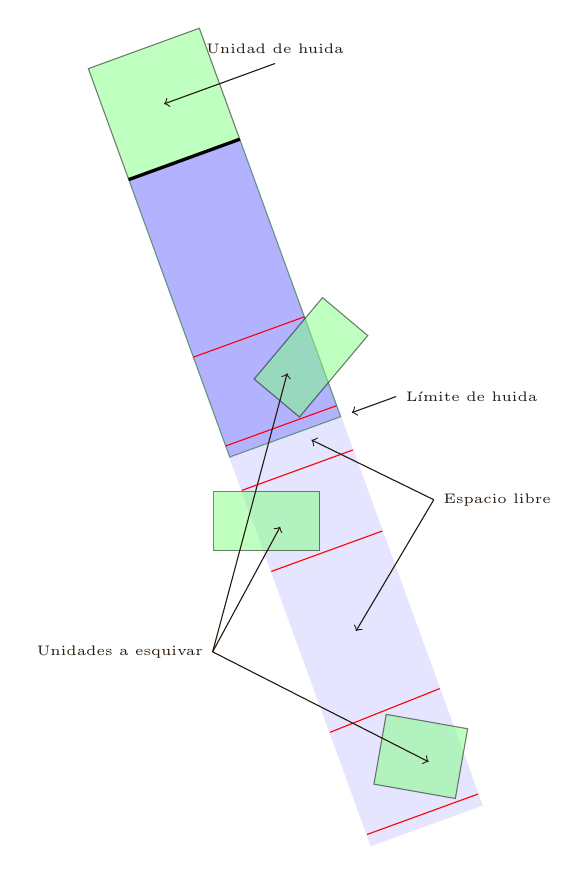
\begin{tikzpicture}[
  scale=1.5,
  rotate=200,
  unidad/.style={opacity=.5,green!50,draw=black},
  area/.style={opacity=.5,blue!50, draw=green!40!black},
  fondo/.style={blue!10},
  descripcion/.style={brown!20!black,->}
  ]

\filldraw[fondo] (0,1) rectangle (1,7);
\filldraw[area] (0,1) rectangle (1,3.5);
\filldraw[unidad] (0,0) rectangle (1,1);
\draw[very thick] (0,1) -- (1,1);
\filldraw[unidad, rotate around={30:(-.2,2.5)}] (-.2,2.5) rectangle
(.7,3);
\filldraw[unidad, rotate around={160:(1.4,4.2)}] (1.4,4.2) rectangle
(2.3,4.7);
\filldraw[unidad, rotate around={150:(.5,6)}] (.5,6) rectangle
(1.2,5.4);

\draw[red] (0,2.6) -- (1,2.6);
\draw[red] (0,3.4) -- (1,3.4);
\draw[red] (0,3.8) -- (1,3.8);
\draw[red] (0,4.53) -- (1,4.53);
\draw[red] (0,5.95) -- (1,5.98);
\draw[red] (0,6.9) -- (1,6.9);

\draw[descripcion] (-.5,.5) node[above]{\tiny{Unidad de huida}} --
(.5,.5);
\draw[descripcion] (-.5,4.43) node[right]{\tiny{Espacio libre}}
-- (.3,3.6);
\draw[descripcion] (-.5,4.43) -- (.5,5.25);
\draw[descripcion] (1.7,5) node[left]{\tiny{Unidades a esquivar}} --
(.3, 6.5);
\draw[descripcion] (1.7,5) -- (.8,4.2);
\draw[descripcion] (1.7,5) -- (.3,3);
\draw[descripcion] (-.5,3.5) node[right]{\tiny{Límite de huida}}--
(-.1,3.5);
\end{tikzpicture}
\end{minipage}